% !TEX root = ./proj_report.tex
\graphicspath{{mehul_pics/}}% Set graphics path location

\chapter{Introduction}
Removing noise from an original signal is a challenging problem receiving due attention from researchers. Digital images play an important role in experimental research and images acquired are often blurry and noisy. Thus prior to analyzing image data, denoising and sharpening becomes necessary. This project aims to explore some of the widely used image enhancement algorithms to sharpen images and implement a robust metric to quantify the performance of filters under different blur sources.\\

\noindent {\bf Mathematical theory behind image processing: }\\
Blurred images are modeled as the true image convolved with a point spread function plus additive noise. The point spread function (PSF) that convolves the true image is generally a property associated with the optics that have contributed to the blur while noise can be due to poor illuminance, quantization among other sources. Mathematically, a blurry image can be represented as follows\\
\begin{equation}
v(m,n)= h(m,n) \star u(m,n) + \eta(m,n)
\end{equation}
where, $u(m,n)$ is the true image, $h(m,n)$ is the PSF, $\eta(m,n)$ is the additive noise and $v(m,n)$ is the blurry image. Image sharpening involves calculating an estimate of the true image $\hat{u}(m,n)$ using filters.
\begin{equation}
\hat{u}(m,n)= g(m,n) \star v(m,n)
\end{equation}
Filters calculate function $g(m,n)$ using some knowledge of the PSF causing the blur and an estimate of the signal to noise ratio.\\

\noindent {\bf Experimental \& Analysis set up: }\\
The experimental and analysis setup for this project is as depicted in the following figure.
\begin{figure}[h!]
  \centering
                \centering
                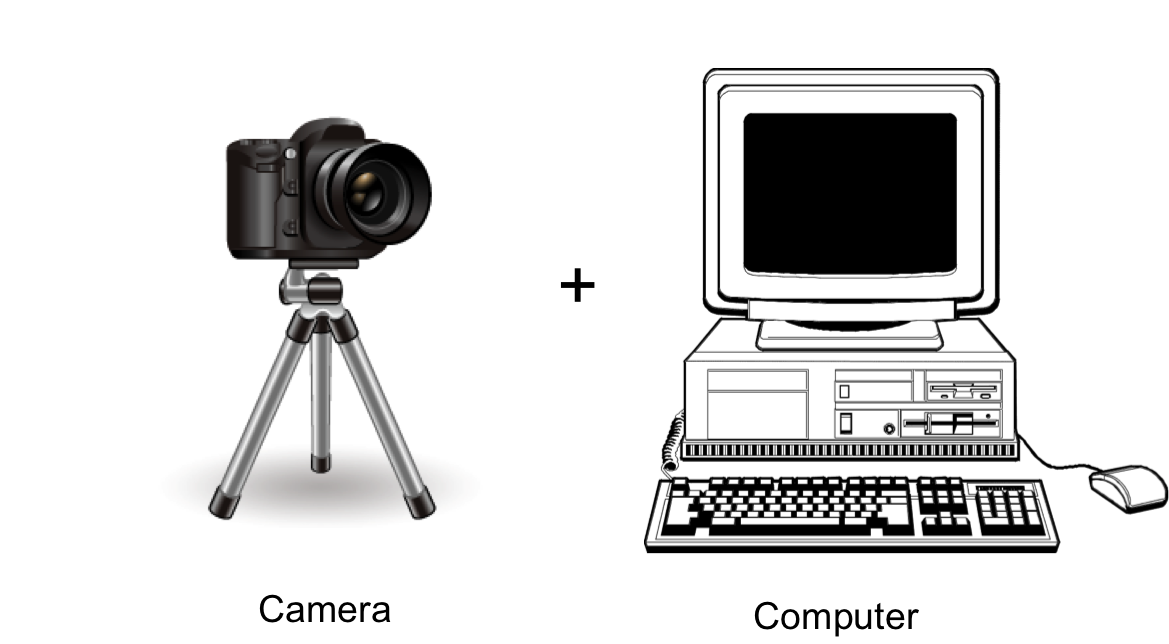
\includegraphics[width=.5\textwidth]{experimental_setup.png}
                \caption{Experimental setup consists of a good camera and a computer system. The camera captures images under pre-defined settings like focal length, shutter speed, aperture size and luminance while computer has been used to perform image enhancement \& filter analysis.}
\end{figure}
\newpage